\documentclass{article}
\usepackage{tikz}
\usetikzlibrary{datavisualization}
\usetikzlibrary{datavisualization.formats.functions}


\usepackage{pgfplots}
\pgfplotsset{width=10cm,compat=1.9}
\usepgfplotslibrary{external}




%\usetikzlibrary{arrows,calc}
%\usetikzlibrary{shapes,positioning}
%\usetikzlibrary{decorations.markings}

\begin{document}
	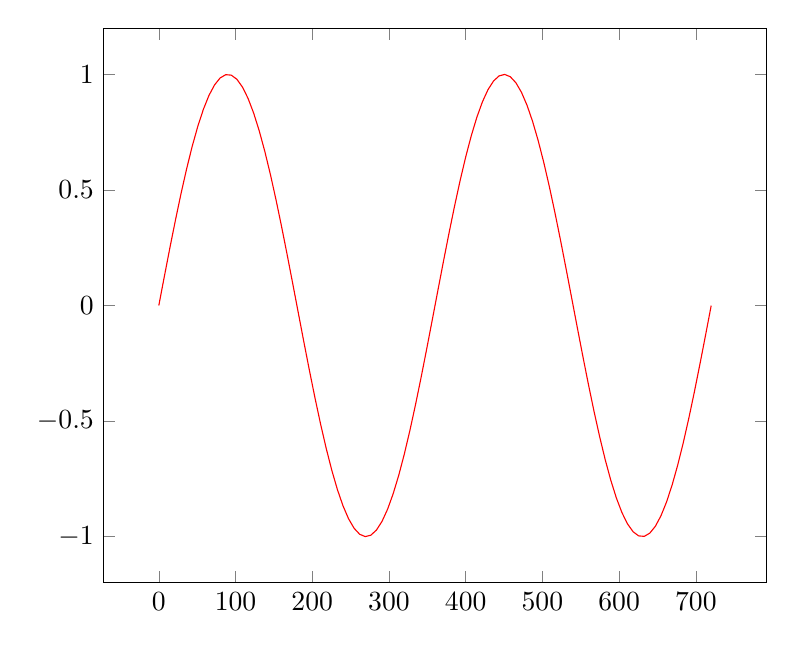
\begin{tikzpicture}
	\begin{axis}
	
	\addplot[color=red,
		domain = 0:2*360,
		samples=100
	]{sin(x)};
	%{sin(deg(x))};
	\end{axis}
	\end{tikzpicture}
\\
	\begin{tikzpicture}
	\begin{axis}[
	title = {Parábola en \LaTeX},
	xlabel = $ x $,
	ylabel = $ f(x) $
	]
	\addplot[
	domain=-10:10,
	color = blue]
	{x^2+4};
	\addlegendentry{$x^2 + 4$}
	
	\addplot[mark=*
	color = red,
	samples=10]
	{exp(x)};
	\addlegendentry{$e^x$}
	\end{axis}	
	\end{tikzpicture}
	
	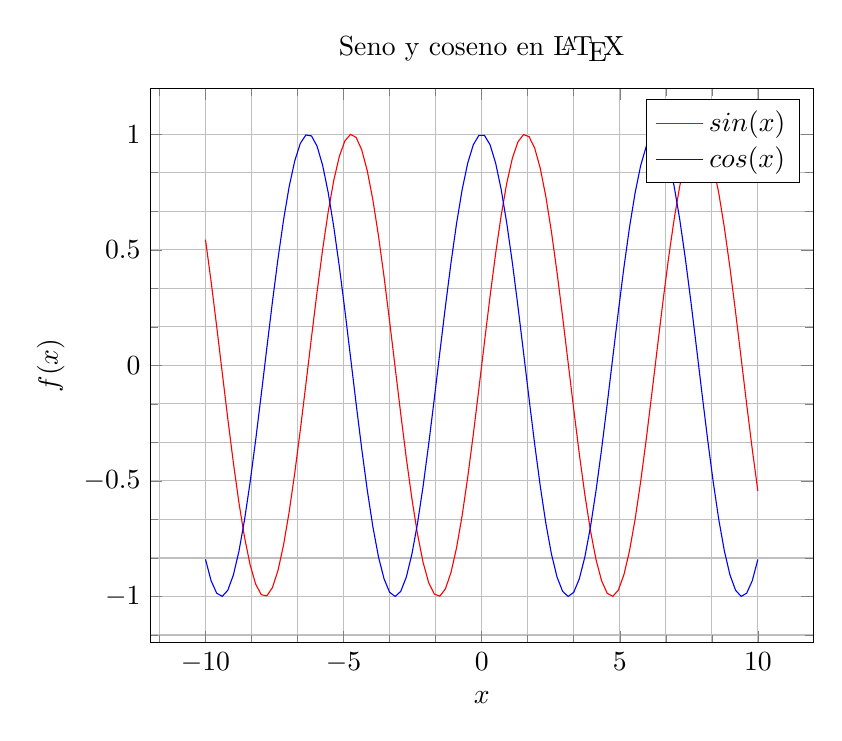
\begin{tikzpicture}
	\begin{axis}[
	title = {Seno y coseno en \LaTeX},
	xlabel = $ x $,
	ylabel = $ f(x) $,
	grid = both, 
	minor tick num=2
	]
	\addplot[
	domain=-10:10,
	samples = 100,
	color = red]
	{sin(deg(x))};
	\addlegendentry{$sin(x)$}

	\addplot[
	domain=-10:10,
	samples = 100,
	color = blue]
	{cos(deg(x))};
	\addlegendentry{$cos(x)$}
	\end{axis}	
	\end{tikzpicture}
	
	\begin{tikzpicture}
		\begin{axis}
		\addplot+ [
		%sharp plot
		%jump mark left
		%jump mark right		
		jump mark mid
		]
		coordinates {(0,0) (1,3) (2,4)};
		\end{axis}
	\end{tikzpicture}
	
	\begin{tikzpicture}
	\begin{axis}[samples=8]
	\addplot+ [
	jump mark left,
	domain=-5:0,
	] {4*x^2 - 5};
	\addplot+ [
	jump mark right,
	domain=-5:0,
	] {0.7*x^3 + 50};
	\end{axis}
	\end{tikzpicture}
	
	
	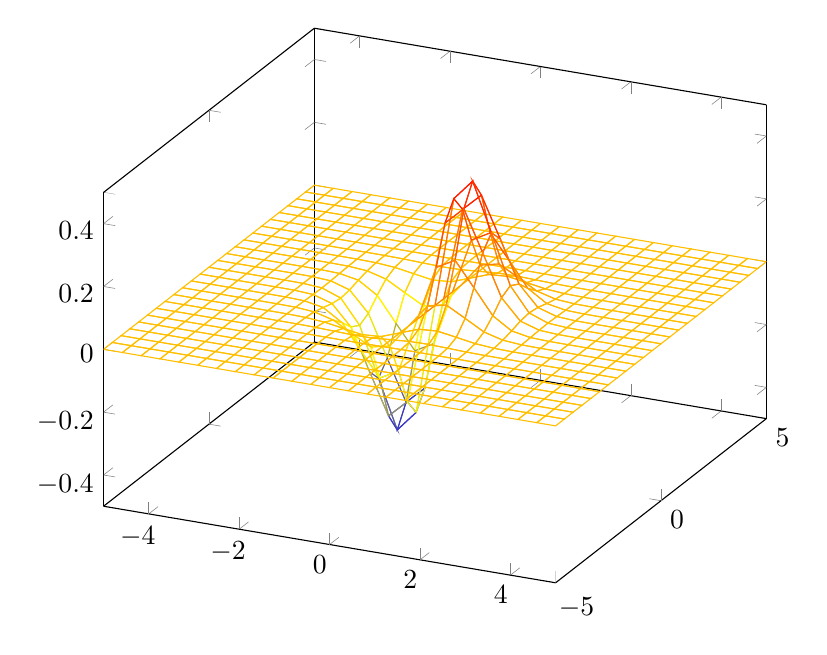
\begin{tikzpicture}
	\begin{axis}
	\addplot3[
	mesh,
%	surf
	]
	{exp(-x^2-y^2)*x};
	\end{axis}
	\end{tikzpicture}
	
	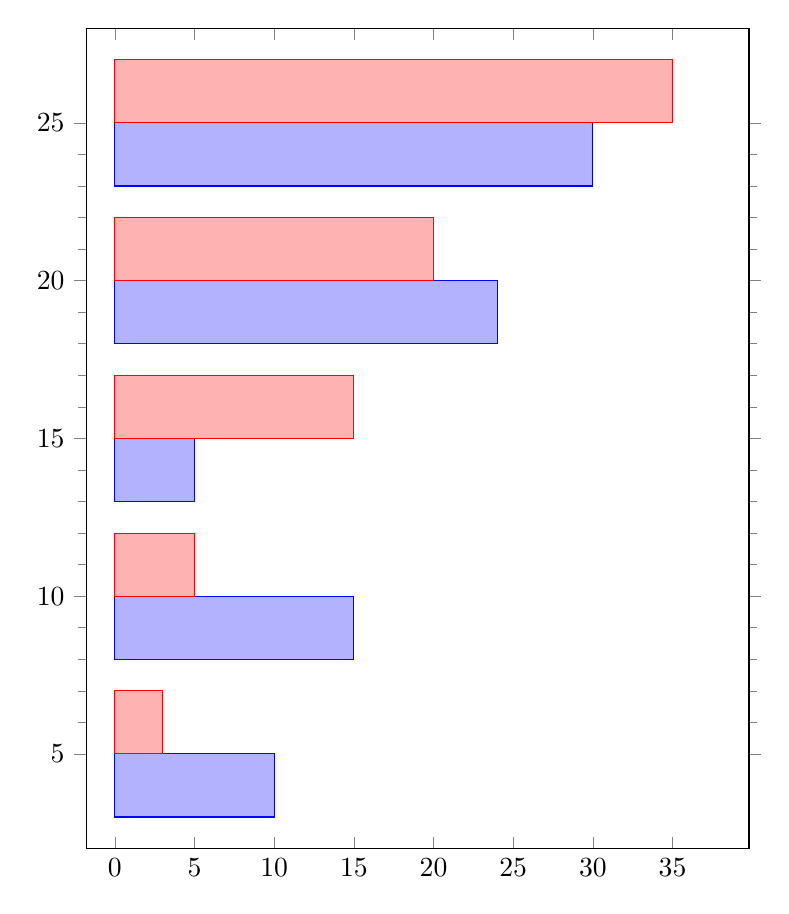
\begin{tikzpicture}
	\begin{axis}[
	xbar=0pt,% space of 0pt between adjacent bars
	bar width=2,
	width=10cm,
	height=12cm,
	minor y tick num=4,
	ytick=data,
	enlargelimits=0.15,
	]
	\addplot coordinates {
		(10,5) (15,10) (5,15) (24,20) (30,25)
	};
	\addplot coordinates {
		(3,5) (5,10) (15,15) (20,20) (35,25)
	};
	\end{axis}
	\end{tikzpicture}
\end{document}